\chapter{Conception de la Solution}

\section*{Introduction du chapitre}
Après avoir défini les besoins fonctionnels et non fonctionnels de notre système de contrôle de la qualité des données, ce chapitre présente la conception détaillée de la solution. Conformément aux exigences du Template 2, nous décrivons dans un premier temps la modélisation dynamique à travers des diagrammes de séquences, et d'activités. Dans un second temps, nous présentons la modélisation statique comprenant le diagramme de classes, le modèle relationnel, le dictionnaire de données et le catalogue complet des règles de qualité. Enfin, nous détaillons l'architecture logicielle (diagramme de composants) et matérielle (diagramme de déploiement) de l'application dans son environnement CIH BANK.

% =========================================================================
\section{Modélisation dynamique}

La modélisation dynamique permet de représenter les interactions temporelles entre les différents composants du système et l'évolution des états des données au cours de l'exécution du processus de contrôle.

\subsection{Diagramme de séquences}
Le diagramme de séquences de la figure \ref{fig:sequence_dq} détaille le flux d'exécution séquentiel d'un scan de qualité de données. Il illustre comment la tâche DQ intégrée dans Airflow coordonne le traitement entre la zone HDFS RAW, le moteur Soda Core et la base Hive de résultats, jusqu'à l'exposition finale vers Tableau.

\begin{figure}[H]
    \centering
    \resizebox{\textwidth}{!}{
    \begin{tikzpicture}[node distance=2.6cm, >=stealth, every node/.style={font=\normalsize}]
        % Lifelines
        \node (airflow) [draw=blue!80!black, fill=blue!10, rounded corners, minimum width=2.2cm, minimum height=1cm, drop shadow] {\textbf{Airflow}};
        \node (sqoop) [draw=blue!80!black, fill=blue!10, rounded corners, minimum width=2.2cm, minimum height=1cm, drop shadow, right=of airflow] {\textbf{Sqoop}};
        \node (hdfs) [draw=blue!80!black, fill=blue!10, rounded corners, minimum width=2.2cm, minimum height=1cm, drop shadow, right=of sqoop] {\textbf{Hive / HDFS}};
        \node (soda) [draw=blue!80!black, fill=blue!10, rounded corners, minimum width=2.5cm, minimum height=1cm, drop shadow, right=of hdfs, align=center] {\textbf{Data Quality}\\\textbf{Engine}};
        \node (dremio) [draw=blue!80!black, fill=blue!10, rounded corners, minimum width=2.2cm, minimum height=1cm, drop shadow, right=of soda] {\textbf{Dremio}};
        \node (tableau) [draw=blue!80!black, fill=blue!10, rounded corners, minimum width=2.2cm, minimum height=1cm, drop shadow, right=of dremio] {\textbf{Tableau}};

        % Dotted lines
        \draw [dashed, draw=gray, thick] (airflow) -- +(0,-18.0);
        \draw [dashed, draw=gray, thick] (sqoop) -- +(0,-18.0);
        \draw [dashed, draw=gray, thick] (hdfs) -- +(0,-18.0);
        \draw [dashed, draw=gray, thick] (soda) -- +(0,-18.0);
        \draw [dashed, draw=gray, thick] (dremio) -- +(0,-18.0);
        \draw [dashed, draw=gray, thick] (tableau) -- +(0,-18.0);

        % Execution arrows
        \draw [->, line width=1.2pt] ($(airflow)+(0,-1.8)$) -- node[above, font=\small, text width=2.4cm, align=center] {1. DAG Ingestion (22h00)} ($(sqoop)+(0,-1.8)$);
        
        \draw [->, line width=1.2pt] ($(sqoop)+(0,-3.3)$) -- node[above, font=\small, text width=2.4cm, align=center] {2. Importer données} ($(hdfs)+(0,-3.3)$);
        
        \draw [<-, dashed, line width=1.2pt, color=green!50!black] ($(sqoop)+(0,-4.8)$) -- node[above, font=\small, text width=2.4cm, align=center] {3. OK (Succès)} ($(hdfs)+(0,-4.8)$);
        
        \draw [->, line width=1.2pt] ($(airflow)+(0,-6.3)$) -- node[above, font=\small, text width=4.5cm, align=center] {4. DAG Qualité (00h00)} ($(soda)+(0,-6.3)$);
        
        \draw [->, line width=1.2pt] ($(soda)+(0,-7.8)$) -- node[above, font=\small, text width=2.4cm, align=center] {5. Évaluer règles sur RAW} ($(hdfs)+(0,-7.8)$);
        
        \draw [<-, dashed, line width=1.2pt, color=gray!80!black] ($(soda)+(0,-9.3)$) -- node[above, font=\small, text width=2.4cm, align=center] {6. Données brutes} ($(hdfs)+(0,-9.3)$);
        
        \draw [->, line width=1.2pt] ($(soda)+(0,-10.8)$) -- node[above, font=\small, text width=2.4cm, align=center] {7. Sauvegarder (3 tables)} ($(hdfs)+(0,-10.8)$);
        
        \draw [->, line width=1.2pt] ($(tableau)+(0,-12.3)$) -- node[above, font=\small, text width=2.4cm, align=center] {8. Requêter le Dashboard} ($(dremio)+(0,-12.3)$);
        
        % Arrow from Dremio to HDFS (crosses Soda)
        \draw [->, line width=1.2pt] ($(dremio)+(0,-13.8)$) -- node[above, font=\small, text width=5cm, align=center, pos=0.7] {9. Interroger les 3 tables} ($(hdfs)+(0,-13.8)$);
        
        % Arrow from HDFS to Dremio (crosses Soda)
        \draw [<-, dashed, line width=1.2pt, color=gray!80!black] ($(dremio)+(0,-15.3)$) -- node[above, font=\small, text width=5cm, align=center, pos=0.7] {10. Virtualisation des données} ($(hdfs)+(0,-15.3)$);
        
        \draw [<-, dashed, line width=1.2pt, color=blue!60!black] ($(tableau)+(0,-16.8)$) -- node[above, font=\small, text width=2.4cm, align=center] {11. Vues consolidées} ($(dremio)+(0,-16.8)$);
        
    \end{tikzpicture}
    }
    \caption{Diagramme de séquences du pipeline de contrôle et restitution DQ}
    \label{fig:sequence_dq}
\end{figure}



\subsection{Diagramme d'activités}
Le diagramme d'activités présenté dans la figure \ref{fig:activity_dq} décrit le processus de bout en bout de traitement de la qualité, depuis le chargement initial des données en zone RAW HDFS jusqu'à la remédiation effective dans l'application source Oracle NOVA.

\begin{figure}[H]
    \centering
    \resizebox{0.9\textwidth}{!}{
    \begin{tikzpicture}[
        >=stealth, 
        every node/.style={font=\normalsize}, 
        block/.style={draw=blue!80!black, rectangle, rounded corners, fill=blue!5, minimum width=4cm, minimum height=1.2cm, align=center, drop shadow, thick}, 
        decision/.style={draw=orange!80!black, diamond, aspect=2.5, fill=yellow!10, minimum width=3cm, minimum height=1.5cm, align=center, drop shadow, thick}
    ]
        % Nodes
        \node (start) [draw, circle, fill=black, inner sep=3pt] at (0,0) {};
        \node (ingest) [block] at (0,-1.5) {\textbf{Ingestion HDFS RAW} \\ (Données Tiers via Sqoop)};
        \node (scan) [block] at (0,-3.3) {\textbf{Exécution Soda Core} \\ (Évaluation des règles DQ)};
        \node (dec) [decision] at (0,-5.5) {\textbf{Anomalies} \\ \textbf{détectées ?}};
        \node (score_ok) [block, fill=green!10, draw=green!60!black] at (6,-5.5) {\textbf{Validation} \\ Score = 100\%};
        \node (score_fail) [block, fill=red!10, draw=red!60!black] at (0,-7.8) {\textbf{Échec (Alerte)} \\ Historisation de l'anomalie};
        \node (remed) [block, fill=purple!10, draw=purple!60!black] at (0,-9.8) {\textbf{Correction Manuelle} \\ (Action par le Data Steward \\ dans Oracle NOVA)};
        \node (end) [draw, circle, double=black, fill=black, inner sep=3pt] at (6,-7.8) {};

        % Arrows
        \draw [->, thick] (start) -- (ingest);
        \draw [->, thick] (ingest) -- (scan);
        \draw [->, thick] (scan) -- (dec);
        \draw [->, thick, color=green!60!black] (dec) -- node[above, font=\small, text=green!60!black, font=\bfseries] {Non (0 erreur)} (score_ok);
        \draw [->, thick, color=red!60!black] (dec) -- node[right, font=\small, text=red!60!black, font=\bfseries] {Oui (> 0)} (score_fail);
        \draw [->, thick] (score_fail) -- (remed);
        \draw [->, thick] (score_ok) -- (end);
        
        % Loop back
        \draw [->, thick, dashed] (remed) .. controls (-4.5,-9.8) and (-4.5,-1.5) .. node[left, font=\small, align=center, xshift=-0.2cm] {Nouveau passage\\(J+1)} (ingest);
    \end{tikzpicture}
    }
    \caption{Diagramme d'activités du workflow de remédiation DQ}
    \label{fig:activity_dq}
\end{figure}

% =========================================================================
\section{Modélisation statique}

La modélisation statique définit la structure fixe du système, ses composants de données, le schéma relationnel de stockage de l'historique de qualité, ainsi que le dictionnaire des métadonnées associées.


\subsection{Modélisation de la table de faits}
Étant donné que la solution s'articule autour de la manipulation de données (Data Management) et non d'un développement orienté objet, nous remplaçons le diagramme de classes traditionnel par une modélisation explicite de la table de faits. 

La figure \ref{fig:fact_dq} illustre la structure des données générée par notre moteur de qualité. Le moteur Soda Core produit un ensemble de trois tables physiques liées par l'identifiant d'exécution (\texttt{run\_id} et \texttt{query\_id}). Ces trois tables sont ensuite unifiées au sein de Dremio pour exposer une grande table de faits consolidée (21 colonnes) servant de source unique de vérité pour le reporting BI.

\begin{figure}[H]
    \centering
    \resizebox{\textwidth}{!}{
    \begin{tikzpicture}[
        every node/.style={font=\small}, 
        tablebox/.style={draw, rectangle split, rectangle split parts=2, fill=blue!5, rounded corners, align=left, drop shadow, text width=5.8cm},
        factbox/.style={draw, rectangle split, rectangle split parts=2, fill=green!10, rounded corners, align=left, drop shadow, text width=6.5cm, line width=1.2pt, draw=green!50!black}
    ]
        
        % Central Fact Table
        \node (fact) [factbox] {
            \centering \textbf{fact\_tiers\_dq\_consolidated} \\ (Vue Dremio - 21 colonnes)
            \nodepart{second}
            \textbf{Clés de jointure :}\\
            - Run\_ID \hfill \textit{String}\\
            - Query\_ID \hfill \textit{String}\\
            \midrule
            \textbf{Indicateurs métier (History) :}\\
            - Date de run \hfill \textit{Date}\\
            - Table \hfill \textit{String}\\
            - Colonne \hfill \textit{String}\\
            - Domaine \hfill \textit{String}\\
            - Règle \hfill \textit{String}\\
            - Score Qualité (\%) \hfill \textit{Double}\\
            - Statut (PASS/WARN/FAIL) \hfill \textit{String}\\
            - Criticité \hfill \textit{String}\\
            - Volume Total \hfill \textit{Long}\\
            - Lignes Conformes \hfill \textit{Long}\\
            \midrule
            \textbf{Configuration (Config) :}\\
            - Requête SQL exécutée \hfill \textit{String}\\
            - Chemin Virtuel Complet \hfill \textit{String}\\
            \midrule
            \textbf{Statuts techniques (Log) :}\\
            - Check Execution Status \hfill \textit{String}\\
            - Check Error Message \hfill \textit{String}\\
            - Run Execution Status \hfill \textit{String}\\
            - Run Error Message \hfill \textit{String}\\
            - Date Mise à jour \hfill \textit{Timestamp}
        };

        % Top Table (History)
        \node (colhist) [tablebox, above=of fact, yshift=1.5cm] {
            \centering \textbf{consolidated\_all\_column\_history} \\ (Table physique Hive)
            \nodepart{second}
            + run\_id \textbf{[PK]} \hfill \textit{String}\\
            + query\_id \textbf{[PK]} \hfill \textit{String}\\
            + colonne\_controlee \hfill \textit{String}\\
            + chemin\_source \hfill \textit{String}\\
            + table\_dataset \hfill \textit{String}\\
            + domaine\_metier \hfill \textit{String}\\
            + type\_regle\_dq \hfill \textit{String}\\
            + volume\_total \hfill \textit{Long}\\
            + lignes\_conformes \hfill \textit{Long}\\
            + score\_qualite\_pct \hfill \textit{Double}\\
            + statut \hfill \textit{String}\\
            + date\_execution \hfill \textit{Timestamp}\\
            + criticite \hfill \textit{String}
        };

        % Bottom Left Table (Checks Config)
        \node (checks) [tablebox, below left=of fact, xshift=-1cm, yshift=-1.5cm] {
            \centering \textbf{consolidated\_all\_checks\_config} \\ (Table physique Hive)
            \nodepart{second}
            + run\_id \textbf{[PK]} \hfill \textit{String}\\
            + query\_id \textbf{[PK]} \hfill \textit{String}\\
            + run\_date \hfill \textit{Date}\\
            + table \hfill \textit{String}\\
            + domain \hfill \textit{String}\\
            + rule \hfill \textit{String}\\
            + virt\_col \hfill \textit{String}\\
            + virt\_full\_path \hfill \textit{String}\\
            + raw\_col \hfill \textit{String}\\
            + sql \hfill \textit{String}\\
            + updated\_at \hfill \textit{Timestamp}\\
            + criticite \hfill \textit{String}
        };

        % Bottom Right Table (Execution Log)
        \node (exec) [tablebox, below right=of fact, xshift=1cm, yshift=-1.5cm] {
            \centering \textbf{consolidated\_execution\_log} \\ (Table physique Hive)
            \nodepart{second}
            + run\_id \textbf{[PK]} \hfill \textit{String}\\
            + query\_id \textbf{[PK]} \hfill \textit{String}\\
            + run\_date \hfill \textit{Date}\\
            + table \hfill \textit{String}\\
            + domain \hfill \textit{String}\\
            + rule \hfill \textit{String}\\
            + virt\_col \hfill \textit{String}\\
            + virt\_full\_path \hfill \textit{String}\\
            + raw\_col \hfill \textit{String}\\
            + check\_execution\_status \hfill \textit{String}\\
            + check\_error\_message \hfill \textit{String}\\
            + check\_timestamp \hfill \textit{Timestamp} \\
            + run\_execution\_status \hfill \textit{String}\\
            + run\_error\_message \hfill \textit{String}\\
            + updated\_at \hfill \textit{Timestamp}
        };

        % Arrows pointing to the central fact table
        \draw[->, line width=1.5pt, draw=gray!80, >=stealth] (colhist.south) -- node[right, font=\footnotesize\bfseries, text=gray!80] {Virtualisation Dremio} (fact.north);
        \draw[->, line width=1.5pt, draw=gray!80, >=stealth] (checks.north east) -- (fact.south west);
        \draw[->, line width=1.5pt, draw=gray!80, >=stealth] (exec.north west) -- (fact.south east);
        
    \end{tikzpicture}
    }
    \caption{Modélisation de la grande table de faits \texttt{fact\_tiers\_dq\_consolidated} et ses 3 tables sources}
    \label{fig:fact_dq}
\end{figure}

\subsection{Modèle relationnel}
Pour persister les résultats d'évaluation de la qualité des données, nous concevons un schéma physique relationnel indépendant au sein de la base de données Hive, basé sur trois tables distinctes :
\begin{itemize}
    \item \textbf{consolidated\_all\_column\_history} : Table principale d'historisation des indicateurs et scores de qualité par exécution, table et colonne. Elle inclut la criticité métier du contrôle.
    \item \textbf{consolidated\_all\_checks\_config} : Table de configuration stockant la requête SQL générée par le moteur pour chaque règle évaluée, ainsi que sa criticité.
    \item \textbf{consolidated\_execution\_log} : Table de journalisation technique traçant le succès ou l'échec d'exécution du contrôle.
\end{itemize}



\subsection{Dictionnaire de données}
Les attributs clés de ces trois tables sont consolidés via Dremio pour fournir un ensemble de 21 colonnes à Tableau. Voici les colonnes principales exploitées :

\begin{table}[H]
\centering
\caption{Dictionnaire simplifié des tables de faits de Qualité des Données}
\label{tab:dict_results_fact}
\renewcommand{\arraystretch}{1.3}
\resizebox{\textwidth}{!}{
\begin{tabular}{|l|l|p{8cm}|}
\hline
\rowcolor{gray!20}
\textbf{Colonne} & \textbf{Table source} & \textbf{Description / Rôle} \\
\hline
\texttt{run\_id} & Toutes & Identifiant unique de l'exécution du processus DQ. \\
\hline
\texttt{query\_id} & Toutes & Identifiant de la requête ou de la règle évaluée. \\
\hline
\texttt{type\_regle\_dq} & \texttt{column\_history} & Dimension DQ (ex: Completude, Conformite, Coherence...). \\
\hline
\texttt{criticite} & \texttt{column\_history} / \texttt{checks\_config} & Niveau de criticité du contrôle (CRITIQUE, HAUTE, MOYENNE). \\
\hline
\texttt{domaine\_metier} & \texttt{column\_history} & Domaine métier visé (PTP-TIE-POR). \\
\hline
\texttt{score\_qualite\_pct} & \texttt{column\_history} & Taux de conformité en pourcentage. \\
\hline
\texttt{statut} & \texttt{column\_history} & État d'évaluation métier de la règle (PASS, WARN, FAIL). \\
\hline
\texttt{sql} & \texttt{checks\_config} & Requête SQL exécutée par le moteur SparkSQL. \\
\hline
\texttt{check\_execution\_status} & \texttt{execution\_log} & Statut d'exécution technique du job (SUCCESS/ERROR). \\
\hline
\end{tabular}
}
\end{table}

\subsection{Catalogue des règles de qualité}
Les contrôles de qualité s'appliquent sur l'ensemble des données du domaine Tiers (informations KYC et données socioprofessionnelles CSP). Afin d'offrir une structuration claire et directement exploitable, le catalogue des règles de gestion est organisé par \textbf{dimension de Data Quality} : Complétude, Conformité, Cohérence, Unicité et Actualité / Pipeline.

L'établissement de ce catalogue découle d'une analyse exploratoire approfondie menée sur un échantillon réel de 5 000 dossiers de personnes physiques issus de la table \texttt{ccm\_npdescription}. Cette analyse a révélé des anomalies typiques et récurrentes de saisie au sein du système opérant Oracle NOVA, ce qui a directement guidé le choix et le paramétrage de nos dimensions de contrôle :
\begin{itemize}
    \item \textbf{Le phénomène des dates de naissance génériques} : Une forte concentration de dates de naissance au premier janvier (\texttt{01/01/YYYY}) a été identifiée (par exemple \texttt{1947-01-01}, \texttt{1961-01-01}), traduisant une saisie par défaut dans NOVA lorsque seule l'année de naissance est connue. Cela justifie notre règle de validité sur \texttt{birthdate} avec un seuil de tolérance de 15\% ,
    \item \textbf{Le codage numérique des villes} : Le champ \texttt{birthcity} contient des codes numériques (comme \texttt{787}) au lieu de libellés textuels, nécessitant un contrôle de validité par rapport au référentiel des villes pour assurer la cohérence et la résolubilité des codes ,
    \item \textbf{La cohérence conditionnelle FATCA} : L'identifiant FATCA (\texttt{fatcaidentificationnumber}) est majoritairement nul, ce qui est cohérent pour les citoyens marocains (\texttt{nationalitycountry = MA}), mais doit être obligatoirement renseigné pour les clients ayant la nationalité ou une double nationalité américaine.
\end{itemize}

\subsubsection{Dimension Complétude}
La dimension de complétude mesure le taux de renseignement des attributs obligatoires pour assurer l'exploitabilité opérationnelle des dossiers clients.

\begin{longtable}{|p{0.20\textwidth}|p{0.30\textwidth}|p{0.14\textwidth}|p{0.30\textwidth}|}
\caption{Dimension Complétude — Données Tiers (KYC \& CSP)} \label{tab:completude_tiers} \\
\hline
\rowcolor{gray!20}
\textbf{Colonne(s)} & \textbf{Description Règle / Seuil} & \textbf{Criticité} & \textbf{Action corrective} \\
\hline
\endfirsthead
\hline
\rowcolor{gray!20}
\textbf{Colonne(s)} & \textbf{Description Règle / Seuil} & \textbf{Criticité} & \textbf{Action corrective} \\
\hline
\endhead
\texttt{name} & 0 valeur nulle tolérée & CRITIQUE & Audit dossiers - Blocage saisie agence \\
\hline
\texttt{firstname} & 0 valeur nulle tolérée & CRITIQUE & Audit dossiers - Blocage saisie agence \\
\hline
\texttt{birthdate} & 0 valeur nulle tolérée & CRITIQUE & Saisie obligatoire avec justificatif officiel \\
\hline
\texttt{nationality\_}\allowbreak\texttt{country} & 0 valeur nulle tolérée & HAUTE & Renseigner le code pays de nationalité \\
\hline
\texttt{professional\_}\allowbreak\texttt{sector} & Taux de valeurs nulles < 5\% & HAUTE & Renseigner le secteur d'activité de l'employeur \\
\hline
\texttt{occupation} & Taux de valeurs nulles < 5\% & HAUTE & Préciser la profession exacte du client \\
\hline
\texttt{socioprofessional\_}\allowbreak\texttt{category} & Taux de valeurs nulles < 5\% & HAUTE & Renseigner la catégorie socioprofessionnelle (CSP) \\
\hline
\texttt{professional\_}\allowbreak\texttt{situation} & Taux de valeurs nulles < 5\% & HAUTE & Renseigner le statut de la situation professionnelle \\
\hline
\texttt{employer} & Taux de valeurs nulles < 10\% & HAUTE & Renseigner le nom de l'entreprise employeuse \\
\hline
\texttt{politically\_}\allowbreak\texttt{exposed} & 0 valeur nulle tolérée (PEP obligatoire) & CRITIQUE & Renseigner la déclaration d'exposition politique \\
\hline
\end{longtable}

\subsubsection{Dimension Conformité}
La dimension de validité évalue le respect des formats de saisie, des plages de valeurs autorisées et la conformité par rapport aux référentiels métier (BAM, ISO).

\begin{longtable}{|p{0.20\textwidth}|p{0.30\textwidth}|p{0.14\textwidth}|p{0.30\textwidth}|}
\caption{Dimension Conformité — Données Tiers (KYC \& CSP)} \label{tab:validite_tiers} \\
\hline
\rowcolor{gray!20}
\textbf{Colonne(s)} & \textbf{Description Règle / Seuil} & \textbf{Criticité} & \textbf{Action corrective} \\
\hline
\endfirsthead
\hline
\rowcolor{gray!20}
\textbf{Colonne(s)} & \textbf{Description Règle / Seuil} & \textbf{Criticité} & \textbf{Action corrective} \\
\hline
\endhead
\texttt{name}, \texttt{firstname} & Longueur $\ge$ 2, aucun chiffre ou caractère spécial & HAUTE & Nettoyage et normalisation dans NOVA \\
\hline
\texttt{birthdate} & Taux de dates génériques au 01/01 < 15\% & HAUTE & Recherche de la date réelle sur pièce d'identité \\
\hline
\texttt{civility} & Valeurs restreintes à (M., MME, MLLE) & HAUTE & Restauration de la valeur selon pièces fournies \\
\hline
\texttt{sex} & Valeurs restreintes à (M, F) & HAUTE & Restauration de la valeur selon pièces fournies \\
\hline
\texttt{birth\_city} & Doit exister dans le référentiel des villes BAM & MOYENNE & Mapping et correction via la table de transcodage \\
\hline
\texttt{professional\_}\allowbreak\texttt{sector} & Code numérique valide dans le référentiel sectoriel & MOYENNE & Transcodage vers les codes officiels BAM \\
\hline
\texttt{professional\_}\allowbreak\texttt{situation} & Valeurs restreintes à (SAL, FON, TRI, AUT, EMP, NDE) & HAUTE & Remplacer par un code référentiel valide \\
\hline
\texttt{employer} & Détection des valeurs parasites ('AUTRE', 'LUI MEME') & HAUTE & Normaliser : mapper 'LUI MEME' vers auto-entrepreneur \\
\hline
\end{longtable}

\subsubsection{Dimension Cohérence}
La dimension de cohérence vérifie l'absence de contradiction logique entre plusieurs attributs interdépendants.

\begin{longtable}{|p{0.20\textwidth}|p{0.30\textwidth}|p{0.14\textwidth}|p{0.30\textwidth}|}
\caption{Dimension Cohérence — Données Tiers (KYC \& CSP)} \label{tab:coherence_tiers} \\
\hline
\rowcolor{gray!20}
\textbf{Colonne(s)} & \textbf{Description Règle / Seuil} & \textbf{Criticité} & \textbf{Action corrective} \\
\hline
\endfirsthead
\hline
\rowcolor{gray!20}
\textbf{Colonne(s)} & \textbf{Description Règle / Seuil} & \textbf{Criticité} & \textbf{Action corrective} \\
\hline
\endhead
\texttt{sex} + \texttt{civility} & Genre M $\neq$ MME/MLLE ; Genre F $\neq$ M. & CRITIQUE & Résolution manuelle des incohérences de saisie \\
\hline
\texttt{fatca\_}\allowbreak\texttt{identification\_}\allowbreak\texttt{number} & Si nationalité ou double nationalité = US, 0 valeur nulle & CRITIQUE & Déclaration réglementaire FATCA immédiate \\
\hline
\texttt{employer} + \texttt{professional\_}\allowbreak\texttt{situation} & Si situation = NDE (sans emploi) ou TRI (retraité), employeur doit être NULL & HAUTE & Annuler le nom d'employeur incohérent dans NOVA \\
\hline
\end{longtable}

\subsubsection{Dimension Unicité}
La dimension d'unicité contrôle l'absence de doublons d'enregistrements et garantit l'unicité des identifiants principaux du référentiel.

\begin{longtable}{|p{0.20\textwidth}|p{0.30\textwidth}|p{0.14\textwidth}|p{0.30\textwidth}|}
\caption{Dimension Unicité — Données Tiers (KYC \& CSP)} \label{tab:unicite_tiers} \\
\hline
\rowcolor{gray!20}
\textbf{Colonne(s)} & \textbf{Description Règle / Seuil} & \textbf{Criticité} & \textbf{Action corrective} \\
\hline
\endfirsthead
\hline
\rowcolor{gray!20}
\textbf{Colonne(s)} & \textbf{Description Règle / Seuil} & \textbf{Criticité} & \textbf{Action corrective} \\
\hline
\endhead
\texttt{oid} / \texttt{radical} & Unicité stricte du numéro de radical client (0 doublon) & CRITIQUE & Fusion des doublons clients dans le référentiel \\
\hline
\texttt{ordnum} & Un seul enregistrement actif principal (\texttt{main=1}) par tiers & HAUTE & Éliminer les contrats de travail multiples actifs \\
\hline
\end{longtable}

\subsubsection{Dimension Actualité et Pipeline}
La dimension de fraîcheur s'assure du bon cadencement de l'ingestion quotidienne et de l'intégrité de la chaîne technique.

\begin{longtable}{|p{0.20\textwidth}|p{0.30\textwidth}|p{0.14\textwidth}|p{0.30\textwidth}|}
\caption{Dimension Actualité et Pipeline — Flux Batch} \label{tab:regles_fraicheur} \\
\hline
\rowcolor{gray!20}
\textbf{Colonne(s)} & \textbf{Description Règle / Seuil} & \textbf{Criticité} & \textbf{Action corrective} \\
\hline
\endfirsthead
\hline
\rowcolor{gray!20}
\textbf{Colonne(s)} & \textbf{Description Règle / Seuil} & \textbf{Criticité} & \textbf{Action corrective} \\
\hline
\endhead
\texttt{batch\_}\allowbreak\texttt{datetime} & Retard d'ingestion HDFS RAW < 26h & HAUTE & Alerte infrastructure Big Data et relance Sqoop \\
\hline
\texttt{row\_count} & Écart de volumétrie entre Oracle NOVA et Hive RAW < 0.1\% & CRITIQUE & Rejouer le DAG d'ingestion Sqoop \\
\hline
\texttt{code\_segment} & Cohérence entre segment client et code\_marche & HAUTE & Recalculer le segment par défaut \\
\hline
\end{longtable}

% =========================================================================
\section{Architecture de l'application}

L'architecture présente la structure logique de la solution DQ et son déploiement physique sur l'infrastructure de production de CIH BANK.

\subsection{Architecture logicielle (diagramme de composants)}
L'architecture logicielle de notre solution s'articule autour de modules découplés. Le diagramme de la figure \ref{fig:components_dq} illustre les interactions entre les modules d'ingestion, de stockage, de contrôle, de virtualisation et de restitution de la solution.

\begin{figure}[H]
    \centering
    \resizebox{\textwidth}{!}{
    \begin{tikzpicture}[>=stealth, every node/.style={font=\small}, box/.style={draw=blue!80!black, rectangle, fill=blue!5, rounded corners, minimum width=2.8cm, minimum height=1cm, align=center, drop shadow}]
        % Orchestrators
        \node (dag_ing) [box, fill=orange!10, draw=orange!60!black] {DAG Ingestion \\ \scriptsize(22h00)};
        \node (dag_dq) [box, fill=orange!10, draw=orange!60!black, below=of dag_ing, yshift=-1.0cm] {Nouveau DAG DQ \\ \scriptsize(00h00)};
        
        % Components
        \node (ingest) [box, right=of dag_ing, xshift=1.5cm] {Module d'Ingestion \\ \scriptsize(Apache Sqoop)};
        \node (lake) [box, right=of ingest, xshift=0.5cm] {Zone de Stockage RAW \\ \scriptsize(Hive / HDFS)};
        
        \node (soda) [box, right=of dag_dq, xshift=1.5cm] {Moteur DQ \\ \scriptsize(Soda Core / Python)};
        \node (res) [box, right=of soda, xshift=0.5cm] {Résultats DQ \\ \scriptsize(Hive / HDFS)};
        
        \node (dremio) [box, below=of res, yshift=-0.5cm] {Couche de Virtualisation \\ \scriptsize(Dremio)};
        \node (tableau) [box, left=of dremio, xshift=-1.5cm] {Dashboard \\ \scriptsize(Tableau)};

        % Connectors
        \draw [->, line width=1pt, dashed, orange!80!black] (dag_ing) -- node[above, font=\scriptsize] {Déclenche} (ingest);
        \draw [->, line width=1pt, dashed, orange!80!black] (dag_dq) -- node[above, font=\scriptsize] {Déclenche} (soda);
        
        \draw [->, line width=1pt, blue!70!black] (ingest) -- node[above, font=\scriptsize] {Écrit} (lake);
        \draw [->, line width=1pt, blue!70!black] (soda) -- node[right, font=\scriptsize, align=center, pos=0.3] {Scan} (lake);
        \draw [->, line width=1pt, blue!70!black] (soda) -- node[above, font=\scriptsize] {Enregistre} (res);
        \draw [->, line width=1pt, blue!70!black] (dremio) -- node[right, font=\scriptsize] {Virtualise} (res);
        \draw [->, line width=1pt, blue!70!black] (tableau) -- node[above, font=\scriptsize] {Requête} (dremio);
    \end{tikzpicture}
    }
    \caption{Diagramme de composants logiciels de la solution DQ}
    \label{fig:components_dq}
\end{figure}

Les composants clés de cette architecture logicielle sont détaillés ci-dessous :

\subsubsection{Conception du moteur DQ — Soda Core}
Le moteur de contrôle s'appuie sur le framework open source Soda Core, spécifiquement la bibliothèque Python \texttt{soda-core} et son connecteur Spark \texttt{soda-core-spark}. Afin d'assurer une exécution optimale dans notre écosystème Big Data, la conception logicielle repose sur les principes d'intégration suivants :
\begin{itemize}
    \item \textbf{Encapsulation PySpark et Vues Temporaires} : Le script d'exécution principal (\texttt{dq\_tiers\_checks.py}) initialise une session Spark locale. Pour chaque table de la zone RAW à contrôler (ex: \texttt{ccm\_npdescription} et \texttt{ccm\_job}), la session Spark charge la table sous forme de DataFrame PySpark, puis l'enregistre en tant que vue temporaire en mémoire via la méthode \texttt{createOrReplaceTempView()}. Cela permet à Soda Core d'exécuter l'analyse de qualité directement sur ces vues mémoire sans poser de verrous ou d'accès concurrents sur les tables Hive physiques ,
    \item \textbf{Définition déclarative des règles (SodaCL)} : Les contrôles de qualité sont externalisés dans des fichiers de règles YAML exploitant le langage déclaratif SodaCL. Les fichiers sont séparés logiquement par domaine : \texttt{checks\_kyc.yml} pour le KYC, \texttt{checks\_csp.yml} pour les données socio-professionnelles, et \texttt{checks\_pipeline.yml} pour les indicateurs techniques et la fraîcheur ,
    \item \textbf{Extraction programmatique et typage des métadonnées} : Après l'exécution du scan, le script Python exploite les structures d'API de Soda Core (l'objet \texttt{Scan}) pour parcourir la liste des vérifications évaluées. Pour chaque règle, le script extrait dynamiquement le résultat (succès/échec), la valeur de la métrique, le seuil, la dimension (Completeness, Validity, Consistency), le domaine et la criticité (définis en tant qu'attributs personnalisés dans le YAML). Un score de conformité sur 100 est attribué pour chaque règle ,
    \item \textbf{Persistance partitionnée dans trois tables Hive} : Après l'exécution du scan, le script consolide les résultats et écrit dans trois tables physiques Hive distinctes : \texttt{consolidated\_all\_column\_history} pour les résultats, \texttt{consolidated\_all\_checks\_config} pour la configuration et les requêtes SQL générées, et \texttt{consolidated\_execution\_log} pour la journalisation technique.
\end{itemize}

\subsubsection{Conception de l'orchestration Airflow}
La planification, le déclenchement et le monitoring des scans de qualité sont gérés par un \textbf{nouveau DAG Airflow indépendant}, spécifiquement dédié au contrôle DQ. Afin de découpler totalement l'ingestion de la vérification de la qualité, ce nouveau DAG est planifié pour s'exécuter quotidiennement à \textbf{00h00}. Cela laisse une marge de sécurité de deux heures après le déclenchement du DAG d'ingestion Sqoop principal (\texttt{dailyow22}, prévu à 22h00). L'architecture d'exécution repose sur un déclenchement direct du moteur d'évaluation Python Soda Core depuis Airflow. Cette séparation modulaire assure qu'une défaillance dans le DAG d'ingestion ne bloque pas ou ne corrompt pas la supervision de la qualité.


\subsubsection{Conception du dashboard Tableau}
La restitution visuelle est structurée dans un dashboard Tableau interactif connecté en direct au dataset virtuel unique de Dremio. L'intelligence analytique (calcul des scores quotidiens moyens, taux de conformité globaux, regroupements par dimension de qualité ou par date) est configurée à l'aide de feuilles de calcul (sheets) et de filtres dynamiques directement dans Tableau Desktop, tirant parti de la table de faits unique. Le dashboard est structuré en quatre onglets fonctionnels :
\begin{enumerate}
    \item \textbf{Vue Exécutive} : Présente les KPIs de conformité globaux et les alertes critiques pour les Data Owners et la Direction ,
    \item \textbf{Détail KYC} : Permet une analyse fine par colonne et par dimension de qualité sur le domaine KYC ,
    \item \textbf{Détail CSP} : Restitue les scores de conformité socioprofessionnelle et l'évaluation des valeurs parasites ,
    \item \textbf{Anomalies \& Remédiation} : Présente une synthèse des règles et colonnes présentant des taux d'anomalies élevés (filtrée sur \texttt{state != 'pass'}), aidant les Data Stewards à cibler les actions correctives collectives dans NOVA.
\end{enumerate}
Pour des raisons évidentes de sécurité et de conformité réglementaire (notamment les directives de Bank Al-Maghrib et la protection des données personnelles), toutes les données nominatives et les radicaux clients affichés dans les onglets opérationnels font l'objet d'un masquage ou d'un floutage systématique, garantissant la stricte confidentialité des informations sensibles.

\begin{figure}[H]
    \centering
    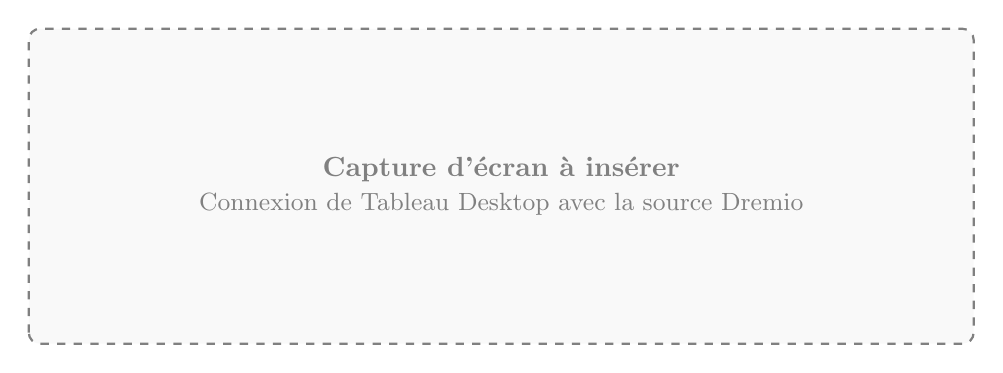
\begin{tikzpicture}
        \draw[draw=gray, dashed, fill=gray!5, thick, rounded corners] (0,0) rectangle (12,4);
        \node at (6,2) [align=center, text=gray] {\textbf{Capture d'écran à insérer} \\ \small Connexion de Tableau Desktop avec la source Dremio};
    \end{tikzpicture}
    \caption{Connexion en direct de Tableau Desktop avec le dataset virtuel Dremio}
    \label{fig:screenshot_tableau_conn}
\end{figure}

\subsection{Architecture matérielle (diagramme de déploiement)}
Le diagramme de déploiement de la figure \ref{fig:deploy_dq} modélise l'architecture système et l'infrastructure distribuée de production sur laquelle est déployée notre solution au sein de CIH BANK.

\begin{figure}[H]
    \centering
    \begin{tikzpicture}[
        node distance=0.8cm and 1.2cm, 
        >=stealth, 
        every node/.style={font=\scriptsize},
        box/.style={
            draw=blue!60!black, 
            fill=blue!5, 
            rounded corners=4pt, 
            minimum width=3.0cm, 
            minimum height=1.1cm, 
            align=center, 
            line width=0.8pt
        }
    ]
        % Nodes
        \node (client) [box] {\textbf{Poste Data Steward} \\ \tiny Tableau Desktop / Web};
        \node (edge) [box, right=of client] {\textbf{Edge Node (Gateway)} \\ \tiny Airflow / Dremio Coordinator \\ \tiny Hive Metastore};
        \node (master) [box, above right=of edge, yshift=-0.3cm] {\textbf{Master Nodes (x3)} \\ \tiny HDFS NameNode \\ \tiny YARN ResourceManager};
        \node (worker) [box, below right=of edge, yshift=0.3cm] {\textbf{Worker Nodes (x3)} \\ \tiny HDFS DataNodes \\ \tiny YARN NodeManagers};

        % Connectors with style
        \draw [<->, thick, blue!80!black] (client) -- (edge);
        \draw [<->, thick, blue!80!black] (edge) -- (master.west);
        \draw [<->, thick, blue!80!black] (edge) -- (worker.west);
        \draw [<->, thick, dashed, gray] (master) -- (worker);
    \end{tikzpicture}
    \caption{Architecture matérielle et déploiement dans le cluster Big Data}
    \label{fig:deploy_dq}
\end{figure}

Le cluster Big Data Cloudera CDP 7.1.7 de production de CIH BANK est structuré autour de 8 nœuds distribués, configurés de la manière suivante :
\begin{itemize}
    \item \textbf{1 Nœud Edge (Gateway) principal} : Ce serveur sert de point d'entrée pour l'administration et l'orchestration des jobs. Il héberge les workers d'Apache Airflow, le coordinateur Dremio, ainsi que le service Hive Metastore. C'est sur ce nœud qu'est installé l'environnement virtuel Python contenant les packages \texttt{soda-core} et \texttt{soda-core-spark} ,
    \item \textbf{3 Nœuds Masters} : Ils assurent la haute disponibilité du stockage (HDFS NameNodes configurés en Actif/Standby et JournalNodes) et la coordination de l'ordonnancement distributed. Ils hébergent également le YARN ResourceManager pour la répartition des ressources du cluster ,
    \item \textbf{3 Nœuds Workers} : Ces serveurs gèrent le stockage local physique sous HDFS (DataNodes) et disposent des YARN NodeManagers pour allouer des conteneurs de calcul lors de l'exécution distribuée de nos requêtes PySpark et Dremio Executors.
\end{itemize}

\subsubsection{Orchestration technique et protocole de sécurité Kerberos}
Afin de sécuriser les accès aux données confidentielles du domaine Tiers de CIH BANK, l'exécution de la solution de qualité s'intègre au protocole de sécurité global du cluster :
\begin{itemize}
    \item \textbf{Authentification Kerberos} : Le cluster Cloudera étant sécurisé par Kerberos, l'autorisation d'accès aux répertoires HDFS RAW nécessite un ticket d'authentification valide. Avant de lancer le traitement, la tâche Airflow utilise le fichier keytab chiffré (\texttt{tiers\_dq.keytab}) associé au compte de service du domaine Tiers (\texttt{tiers\_dq\_service}) pour générer et renouveler automatiquement le ticket Kerberos via la commande système \texttt{kinit} ,
    \item \textbf{Soumission du job Spark sur YARN} : Le script Python principal est exécuté en mode \texttt{spark-submit} avec le gestionnaire de ressources YARN configuré en mode \texttt{client} depuis le nœud Edge. Le driver Spark s'exécute ainsi localement sur le Gateway Node (dans le process Airflow), tandis que YARN ResourceManager alloue de manière distribuée des exécuteurs Spark au sein des nœuds Workers. Ces exécuteurs lisent et traitent en parallèle les partitions des fichiers HDFS de la zone RAW Hive.
\end{itemize}

% =========================================================================
\subsection{Technologies de l'écosystème utilisées}

Pour s'insérer au mieux au sein du système d'information décisionnel et Big Data de CIH BANK, notre solution exploite les briques technologiques de l'écosystème du Data Lake. Ces technologies sont résumées ci-dessous.

\vspace{0.4cm}

\noindent
\begin{minipage}[c]{0.12\textwidth}
    \centering
    
\includegraphics[width=\textwidth, height=1.0cm, keepaspectratio]{figures/logos/logo_oracle.png}
\end{minipage}
\hspace{0.03\textwidth}
\begin{minipage}[c]{0.83\textwidth}
    \textbf{Oracle NOVA} --- Système opérant source\\
    {\small Base de données relationnelle hébergeant le Core Banking de la banque. Il s'agit du point d'entrée unique des données des clients physiques et moraux (Référentiel Tiers) et de la cible finale de correction.}
\end{minipage}

\vspace{0.4cm}\noindent\rule{\textwidth}{0.2pt}\vspace{0.3cm}

\noindent
\begin{minipage}[c]{0.12\textwidth}
    \centering
    
\includegraphics[width=\textwidth, height=1.0cm, keepaspectratio]{figures/logos/logo_sqoop.png}
\end{minipage}
\hspace{0.03\textwidth}
\begin{minipage}[c]{0.83\textwidth}
    \textbf{Apache Sqoop} --- Ingestion batch Oracle vers HDFS\\
    {\small Technologie d'ingestion permettant le transfert en masse des tables NOVA vers l'infrastructure Hadoop de manière planifiée.}
\end{minipage}

\vspace{0.4cm}\noindent\rule{\textwidth}{0.2pt}\vspace{0.3cm}

\noindent
\begin{minipage}[c]{0.12\textwidth}
    \centering
    
\includegraphics[width=\textwidth, height=1.0cm, keepaspectratio]{figures/logos/logo_airflow.png}
\end{minipage}
\hspace{0.03\textwidth}
\begin{minipage}[c]{0.83\textwidth}
    \textbf{Apache Airflow} --- Orchestrateur de tâches\\
    {\small Outil d'orchestration permettant de planifier, ordonnancer et superviser l'exécution du flux d'ingestion et des scans de qualité de manière centralisée.}
\end{minipage}

\vspace{0.4cm}\noindent\rule{\textwidth}{0.2pt}\vspace{0.3cm}

\noindent
\begin{minipage}[c]{0.12\textwidth}
    \centering
    
\includegraphics[width=\textwidth, height=1.0cm, keepaspectratio]{figures/logos/logo_hadoop.png}
\end{minipage}
\hspace{0.03\textwidth}
\begin{minipage}[c]{0.83\textwidth}
    \textbf{HDFS / Apache Hive} --- Plateforme de stockage et de requêtage\\
    {\small HDFS assure le stockage persistant distribué tandis que Hive structure ces répertoires sous forme de tables SQL relationnelles cibles pour nos contrôles.}
\end{minipage}

\vspace{0.4cm}\noindent\rule{\textwidth}{0.2pt}\vspace{0.3cm}

\noindent
\begin{minipage}[c]{0.12\textwidth}
    \centering
    
\includegraphics[width=\textwidth, height=1.0cm, keepaspectratio]{figures/logos/logo_soda.png}
\end{minipage}
\hspace{0.03\textwidth}
\begin{minipage}[c]{0.83\textwidth}
    \textbf{Soda Core} --- Moteur de contrôle de la qualité (Python)\\
    {\small Framework de validation de données déclaratif basé sur des fichiers YAML de règles de gestion et exécuté programmatiquement sur les tables Hive RAW.}
\end{minipage}

\vspace{0.4cm}\noindent\rule{\textwidth}{0.2pt}\vspace{0.3cm}

\noindent
\begin{minipage}[c]{0.12\textwidth}
    \centering
    
\includegraphics[width=\textwidth, height=1.0cm, keepaspectratio]{figures/logos/logo_dremio.png}
\end{minipage}
\hspace{0.03\textwidth}
\begin{minipage}[c]{0.83\textwidth}
    \textbf{Dremio} --- Moteur de virtualisation et d'exposition\\
    {\small Permet de virtualiser les tables de résultats Hive et d'exposer des vues SQL rapides et sécurisées, éliminant le besoin de dupliquer ou de transférer physiquement les volumes de données.}
\end{minipage}

\vspace{0.4cm}\noindent\rule{\textwidth}{0.2pt}\vspace{0.3cm}

\noindent
\begin{minipage}[c]{0.12\textwidth}
    \centering
    
\includegraphics[width=\textwidth, height=1.0cm, keepaspectratio]{figures/logos/logo_tableau.png}
\end{minipage}
\hspace{0.03\textwidth}
\begin{minipage}[c]{0.83\textwidth}
    \textbf{Tableau} --- Outil d'analyse décisionnelle et Visualisation\\
    {\small Solution BI standard de CIH BANK, connectée en direct à Dremio pour fournir un reporting réactif sur la qualité des tiers à l'intention des Data Owners.}
\end{minipage}

\vspace{0.4cm}

% =========================================================================
\section*{Conclusion du chapitre}
Ce chapitre a décrit la conception complète de la solution de contrôle de la qualité du domaine Tiers. Nous avons structuré la dynamique d'exécution de nos scans et le cycle de vie des anomalies identifiées. La modélisation statique a fourni le diagramme de classes de nos indicateurs, le schéma relationnel et le catalogue complet des règles KYC et CSP de la solution. Enfin, l'architecture logicielle (composants) et matérielle (déploiement) a été détaillée au sein de l'environnement de production. Le chapitre suivant présente l'implémentation physique et les résultats opérationnels obtenus.
